\section{DFDs}
A data flow diagram (DFD) is a graphical representation of the "flow" of data through an information system, modeling its process aspects. A DFD is often used as a preliminary step to create an overview of the system, which can later be elaborated. DFDs to serve a tile is as following-:
\begin{figure}[h!]
\centering
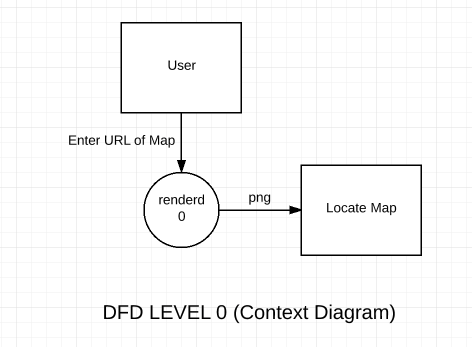
\includegraphics[scale=0.6]{input/images/DFD_0.png}
\caption{Data Flow Diagram Level 0}
\end{figure}
\begin{figure}[h!]
	\centering
	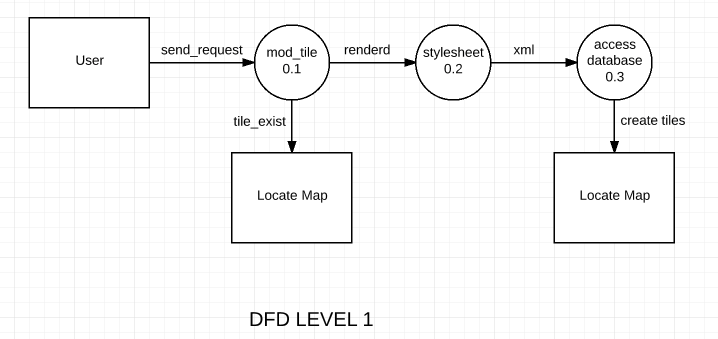
\includegraphics[scale=0.6]{input/images/DFD_1.png}
	\caption{Data Flow Diagram Level 1}
\end{figure}
\begin{figure}[h!]
	\centering
	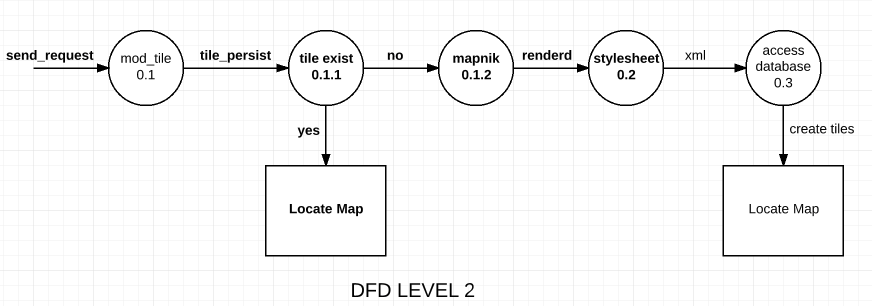
\includegraphics[scale=0.6]{input/images/DFD_2.png}
	\caption{Data Flow Diagram Level 2}
\end{figure}

\section{Flowchart}
A flowchart is a type of diagram that represents an algorithm, work flow or process, showing the steps as boxes of various kinds, and their order by connecting them with arrows
and following are flowchart of showing flow of control and Data in the software-:

\begin{figure}[h!]
	\centering
	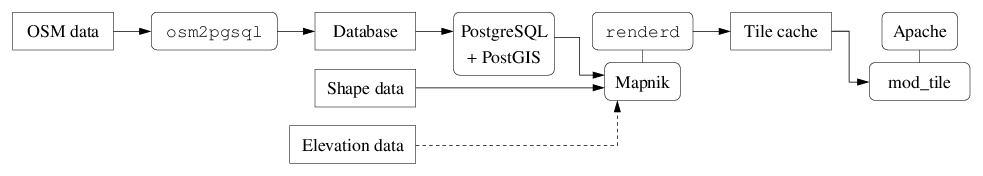
\includegraphics[scale=0.6]{input/images/osmserv.png}
	\caption{Data Flow Of Whole System}
\end{figure}



\begin{figure}[h!]
\centering
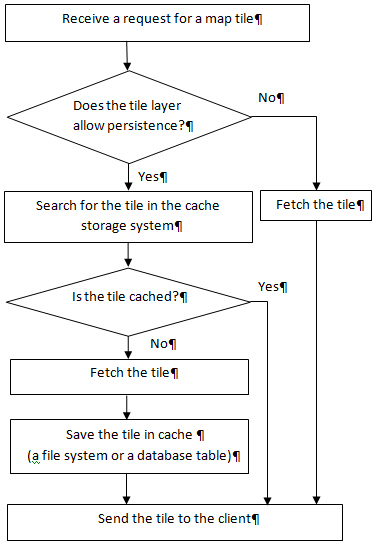
\includegraphics[scale=0.9]{input/images/fetch.jpg}
\caption{Flow Chart to Serve a Tile}
\end{figure}
\hspace{-1.7em}



\section{Problem Formulation}
Geographical data (geo data) is not free in many parts of the world.\\
Because that data is copyrighted and owned by multiple organisations like the Ordnance Survey. Google/whoever just licenses it. If we were to use it, we'd have to pay for it. \\
\noindent "OpenStreetMap is a free editable map of the whole world. It is made by people like you." Which means the database will always be subject to the whims, experimentation, and mistakes of the community. This is precisely OSM's strength since, among other things, it allows our data to quickly accommodate changes in the physical world.\\
\noindent By making your system an OSM tile server not only you can edit the map but can use it offline also. You can change the styling of the map like color of the roads fonts style and amny more as per your requirments. 


\section{Dependencies}
%\subsection{Hardware Requirements}
\begin{itemize}
\item Operating System: Linux/Windows
\item Processor Speed: 512KHz or more
\item RAM: Minimum 2GB
\item Library: Mapnik
\item Modules: Mod\_tile
\item Compiler: CartoCSS
\item Stylesheet: OSMBright
\item Programming Language: C++, Python
\end{itemize}
%\subsection{Software Requirements}
%\begin{itemize}
%\item Library: Mapnik
%\item Modules: Mod\_tile
%\item Compiler: CartoCSS
%\item Stylesheet: OSMBright 
%\item Programming Language: C++, Python 
%\end{itemize}

\section{Methodology}
\begin{itemize}
\item Studying various methods available to solve different problems of numerical analysis.
\item Deciding various input and output parameters of methods.
\item Making the approach modular 
\item Styling the map.
\item Generating documentation
\end{itemize}

\section{Project Work} 
\textbf{Studied Previous System:}\\
Before starting the project, \\\\
\textbf{Learn Linux:}\\
Before starting with project, we have to install various things to make our system an OSM server. So, for that you should know terminal commands because I gonna explain it for Ubuntu only. It is possible on other OS also but you have to work it own. I have provided some basic command also for Linux. \\\\
\textbf{Learn Postgresql:}\\
 We have to go through the basics of postgresql(database) also, such that there
should not be any problem proceeding with project.\\\\
\textbf{Make or Cmake}\\
The softwares like mapnik, mod\_tile, osm2pqsql, are compiled through the Cmake which is basically language. So, we should the basics of it.
\\\\
\textbf{Languages:}\\
We should the basics of the languages like C++, javascript, python etc for manuplating the stylying and rendering of the map.\\\\
\textbf{Input:}\\
Input values are taken from user or default values defined in the file are used.\\\\
\textbf{Output:}\\
According to input values we will get the particular location of the map.

